\section{Diagramme d'enseignement}

\par On pr�sente ici la gestion des enseignements. Elle regroupe
�galement les paquetages de la section et de mati�re.\\

\begin{itemize}
\item TeachingManager : C'est l'objet qui g�re les enseignements, il
s'occupe de leur cr�ation, recherche, mise dans la corbeille,
restauration  et suppression.\\

\item TeachingData : Il s'occupe du stockage des enseignements dans
leur int�gralit�. Le teachingManager lui fait appel pour toutes les
op�rations.\\

\item TeachingTrash : C'est l'objet qui collecte tous les
enseignements mis � la poubelle pour leur cr�ateurs. Il les conserve
jusqu'a leur suppression.\\

\item SectionManager : Il g�re l'ensemble des sections et int�ragit
avec le TeachingManager lors de la cr�ation ou de la recherche.\\

\item UnitManager : Il s'occupe des mati�re et int�ragit
avec le TeachingManager lors de la cr�ation ou de la recherche.\\
\end{itemize}

\begin{center}
\scalebox{0.6}{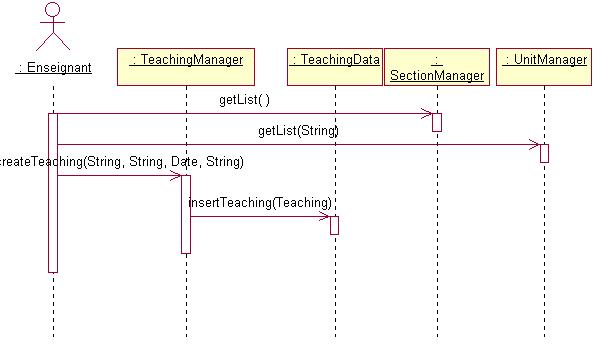
\includegraphics{images/creerEnseignement.jpg}}\\
\par Voici le diagramme de s�quence de cr�ation d'enseignement.\\

\scalebox{0.6}{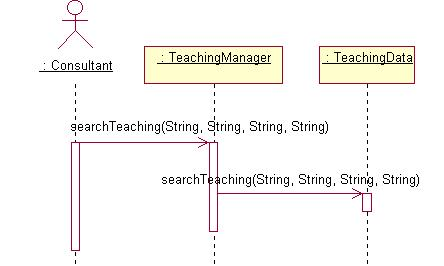
\includegraphics{images/rechercherEns.jpg}}\\
\par Voici le diagramme de s�quence de recherche d'enseignement.\\

\scalebox{0.6}{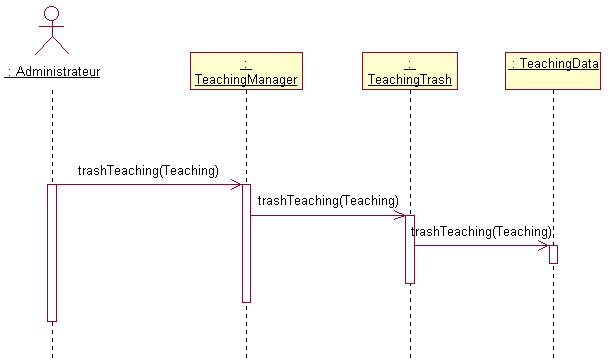
\includegraphics{images/mettreEnsCorbeille.jpg}}\\
\par Voici le diagramme de s�quence de mise � la corbeille
d'enseignement.\\

\scalebox{0.6}{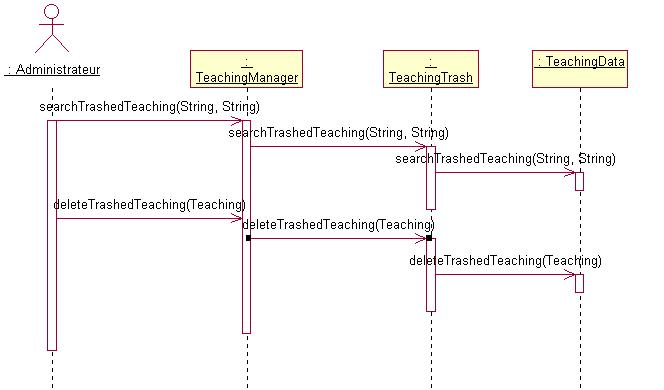
\includegraphics{images/supprimerEns.jpg}}\\
\par Voici le diagramme de s�quence de la suppression d'enseignement.\\


\end{center}




